\section{Integrating Factors}

\noindent
In  Section~2.5 we saw that if $M$, $N$, $M_y$ and $N_x$ are
continuous and $M_y=N_x$ on an open rectangle $R$ then
\begin{equation} \label{eq:2.6.1}
M(x,y)\,dx+N(x,y)\,dy=0
\end{equation}
is exact on $R$. Sometimes an equation that isn't  exact can be made
exact by multiplying it by an appropriate function. For example,
\begin{equation}\label{eq:2.6.2}
(3x+2y^2)\,dx+2xy\,dy=0
\end{equation}
is  not exact, since
$M_y(x,y)=4y\ne  N_x(x,y)=2y$ in \eqref{eq:2.6.2}.
 However, multiplying \eqref{eq:2.6.2}  by $x$ yields
\begin{equation}\label{eq:2.6.3}
(3x^2+2xy^2)\,dx+2x^2y\,dy=0,
\end{equation}
which is exact, since
$M_y(x,y)=N_x(x,y)=4xy$ in \eqref{eq:2.6.3}.
Solving \eqref{eq:2.6.3} by the procedure given in  Section~2.5
 yields the implicit solution
$$
x^3+x^2y^2=c.
$$

A function $\mu=\mu(x,y)$ is  an {\color{blue}\it integrating factor} for
\eqref{eq:2.6.1}  if
\begin{equation}\label{eq:2.6.4}
 \mu(x,y)M (x,y)\,dx+\mu(x,y)N (x,y)\,dy=0
 \end{equation}
 is exact. If we know an integrating
factor $\mu$ for \eqref{eq:2.6.1}, we can solve the exact equation
\eqref{eq:2.6.4} by the method of Section~2.5. It would be
nice
if we could say that \eqref{eq:2.6.1} and \eqref{eq:2.6.4} always have the
same solutions, but this isn't so. For example, a solution
$y=y(x)$ of \eqref{eq:2.6.4} such that $\mu(x,y(x))=0$ on some interval
$a<x<b$ could fail to be a solution of \eqref{eq:2.6.1}
(Exercise~\ref{exer:2.6.1}), while
\eqref{eq:2.6.1} may have a solution $y=y(x)$ such that $\mu(x,y(x)) $
isn't even defined (Exercise~\ref{exer:2.6.2}). Similar comments
apply if $y$ is the independent variable and $x$ is the dependent
variable  in \eqref{eq:2.6.1} and \eqref{eq:2.6.4}.  However, if $\mu(x,y)$
is defined and nonzero for all $(x,y)$,  \eqref{eq:2.6.1}  and
\eqref{eq:2.6.4} are equivalent; that is, they have the same solutions.

\boxit{Finding Integrating Factors}

\noindent
By applying Theorem~\ref{thmtype:2.5.2} (with $M$ and $N$ replaced by $\mu M$
and $\mu N$), we see that \eqref{eq:2.6.4} is exact on an open rectangle
$R$ if $\mu M$, $\mu N$, $(\mu M)_y$, and $(\mu N)_x$ are continuous
and
$$
{\partial\over\partial y}(\mu M)={\partial\over\partial x}
(\mu N) \mbox{\quad or, equivalently, \quad}
\mu_yM+\mu M_y=\mu_xN+\mu N_x
$$
on $R$. It's better to rewrite the last equation as
\begin{equation} \label{eq:2.6.5}
\mu(M_y-N_x)=\mu_xN-\mu_yM,
\end{equation}
which  reduces to  the known result for exact equations;
that is, if $M_y=N_x$ then \eqref{eq:2.6.5} holds with $\mu=1$, so
\eqref{eq:2.6.1} is exact.

You may think  \eqref{eq:2.6.5} is of little value, since it involves
{\color{blue}\it partial\/} derivatives of the unknown integrating factor $\mu$,
and we haven't studied methods for solving such equations. However,
we'll now show that \eqref{eq:2.6.5} is useful if we restrict our search
to integrating factors that are products of a function of
$x$ and a function of $y$; that is,
$\mu(x,y)=P(x)Q(y)$.
We're not saying that {\color{blue}\it every\/} equation
 $M\,dx+N\,dy=0$ has an integrating factor of this
form;   rather, we're saying that {\color{blue}\it some\/} equations have
such integrating
factors. We'll now develop a way to determine whether a given
equation has such an integrating factor, and a method for finding the
integrating factor in this case.

If $\mu(x,y)=P(x)Q(y)$, then $\mu_x(x,y)=P'(x)Q(y)$ and
$\mu_y(x,y)=P(x)Q'(y)$, so \eqref{eq:2.6.5} becomes
\begin{equation} \label{eq:2.6.6}
P(x)Q(y)(M_y-N_x)=P'(x)Q(y)N-P(x)Q'(y)M,
\end{equation}
or, after dividing through by $P(x)Q(y)$,
\begin{equation} \label{eq:2.6.7}
M_y-N_x={P'(x)\over P(x)}N-{Q'(y)\over Q(y)}M.
\end{equation}
Now let
$$
p(x)={P'(x)\over P(x)} \mbox{\quad and \quad} q(y)={Q'(y)\over Q(y)},
$$
so \eqref{eq:2.6.7} becomes
\begin{equation} \label{eq:2.6.8}
M_y-N_x=p(x)N-q(y)M.
\end{equation}

We obtained \eqref{eq:2.6.8} by {\color{blue}\it assuming\/} that $M\,dx+N\,dy=0$ has
an integrating factor $\mu(x,y)=P(x)Q(y)$. However, we can
now view \eqref{eq:2.6.7} differently: If there are functions $p=p(x)$
and $q=q(y)$  that satisfy \eqref{eq:2.6.8} and we define
\begin{equation} \label{eq:2.6.9}
P(x)=\pm e^{\int p(x)\,dx}\mbox{\quad and \quad}
Q(y)=\pm e^{\int q(y)\,dy},
\end{equation}
then reversing the steps that led from \eqref{eq:2.6.6} to
\eqref{eq:2.6.8} shows that $\mu(x,y)=P(x)Q(y)$ is an integrating factor
for $M\,dx+N\,dy=0$. In using this result, we take the constants of
integration in \eqref{eq:2.6.9} to be zero and choose the signs
conveniently so the integrating factor has the simplest form.

There's no simple general method for ascertaining
whether functions $p=p(x)$ and $q=q(y)$ satisfying \eqref{eq:2.6.8}
exist. However, the next theorem gives simple sufficient
conditions for the given equation to have an integrating factor that
depends on only one of the independent variables $x$ and $y$, and for
finding an integrating factor in this case.

\begin{theorem}\color{blue}\label{thmtype:2.6.1}
Let $M,$ $N,$ $M_y,$ and $N_x$ be continuous on an open rectangle $R.$
Then$:$
\begin{alist}
\item % (a)
 If $(M_y-N_x)/N$ is independent
of $y$ on $R$ and  we define
$$
p(x)={M_y-N_x\over N}
$$
 then
\begin{equation}\label{eq:2.6.10}
\mu(x)=\pm e^{\int p(x)\,dx}
\end{equation}
is an integrating factor for
\begin{equation}\label{eq:2.6.11}
M(x,y)\,dx+N(x,y)\,dy=0
\end{equation}
on $R.$
\item % (b)
If $(N_x-M_y)/M$ is independent of $x$ on
$R$ and we define
$$
q(y)={N_x-M_y\over M},
$$
then
\begin{equation}\label{eq:2.6.12}
\mu(y)=\pm e^{\int q(y)\,dy}
\end{equation}
 is an integrating factor for \eqref{eq:2.6.11} on $R.$
\end{alist}
\end{theorem}

\medskip

\proof (a)
If $(M_y-N_x)/N$ is independent of $y$, then \eqref{eq:2.6.8}
 holds with $p=(M_y-N_x)/N$ and $q\equiv0$. Therefore
 $$
P(x)=\pm e^{\int p(x)\,dx}\mbox{\quad and\quad}Q(y)=\pm e^{\int
q(y)\,dy}=\pm e^0=\pm1,
 $$
so \eqref{eq:2.6.10} is an integrating factor for \eqref{eq:2.6.11} on $R$.

(b) If $(N_x-M_y)/M$ is independent of $x$ then eqref{eq:2.6.8} holds
with $p\equiv0$ and $q=(N_x-M_y)/M$, and a similar argument shows that
\eqref{eq:2.6.12} is an integrating factor for \eqref{eq:2.6.11} on $R$.\bbox

The next two examples show how to apply
Theorem~\ref{thmtype:2.6.1}.

\begin{example}\label{example:2.6.1}
\rm  Find an integrating factor for the equation
\begin{equation}\label{eq:2.6.13}
(2xy^3-2x^3y^3-4xy^2+2x)\,dx+(3x^2y^2+4y)\,dy=0
\end{equation}
and solve the equation.
\end{example}

\solution In \eqref{eq:2.6.13}
$$
M=2xy^3-2x^3y^3-4xy^2+2x,\ N=3x^2y^2+4y,
$$
and
$$
M_y-N_x=(6xy^2-6x^3y^2-8xy)-6xy^2=-6x^3y^2-8xy,
$$
so \eqref{eq:2.6.13}  isn't  exact. However,
$$
{M_y-N_x\over N}=-{6x^3y^2+8xy\over
3x^2y^2+4y}=-2x
$$
is independent of $y$, so Theorem~\ref{thmtype:2.6.1}\part{a} applies
with
$p(x)=-2x$. Since
$$
\int p (x)\,dx=-\int 2x\,dx=-x^2,
$$
 $\mu(x)=e^{-x^2}$ is an
integrating factor.  Multiplying \eqref{eq:2.6.13} by $\mu$ yields the
exact equation
\begin{equation}\label{eq:2.6.14}
e^{-x^2}(2xy^3-2x^3y^3-4xy^2+2x)\,dx+
 e^{-x^2}(3x^2y^2+4y)\,dy=0.
\end{equation}

To solve this equation, we must find a
function $F$ such that
\begin{equation}\label{eq:2.6.15}
F_x(x,y)=e^{-x^2}(2xy^3-2x^3y^3-4xy^2+2x)
\end{equation}
 and
\begin{equation}\label{eq:2.6.16}
F_y(x,y)=e^{-x^2}(3x^2y^2+4y).
\end{equation}
 Integrating \eqref{eq:2.6.16} with respect to $y$ yields
\begin{equation}\label{eq:2.6.17}
F(x,y)=e^{-x^2}(x^2y^3+2y^2)+\psi(x).
\end{equation}
 Differentiating this with respect to $x$ yields
$$
F_x(x,y)=e^{-x^2}(2xy^3-2x^3y^3-4xy^2)+\psi'(x).
$$
Comparing this with \eqref{eq:2.6.15} shows that $\psi'(x)=
2xe^{-x^2}$;  therefore, we can let $\psi(x)=-e^{-x^2}$ in
\eqref{eq:2.6.17} and conclude that
$$
e^{-x^2}\left(y^2(x^2y+2)-1\right)=c
$$
is an implicit solution of \eqref{eq:2.6.14}. It is also an implicit solution
of \eqref{eq:2.6.13}.

Figure~\ref{figure:2.6.1}  shows a  direction field and some integral curves
for \eqref{eq:2.6.13}

  \begin{figure}[tbp]
  \centering
  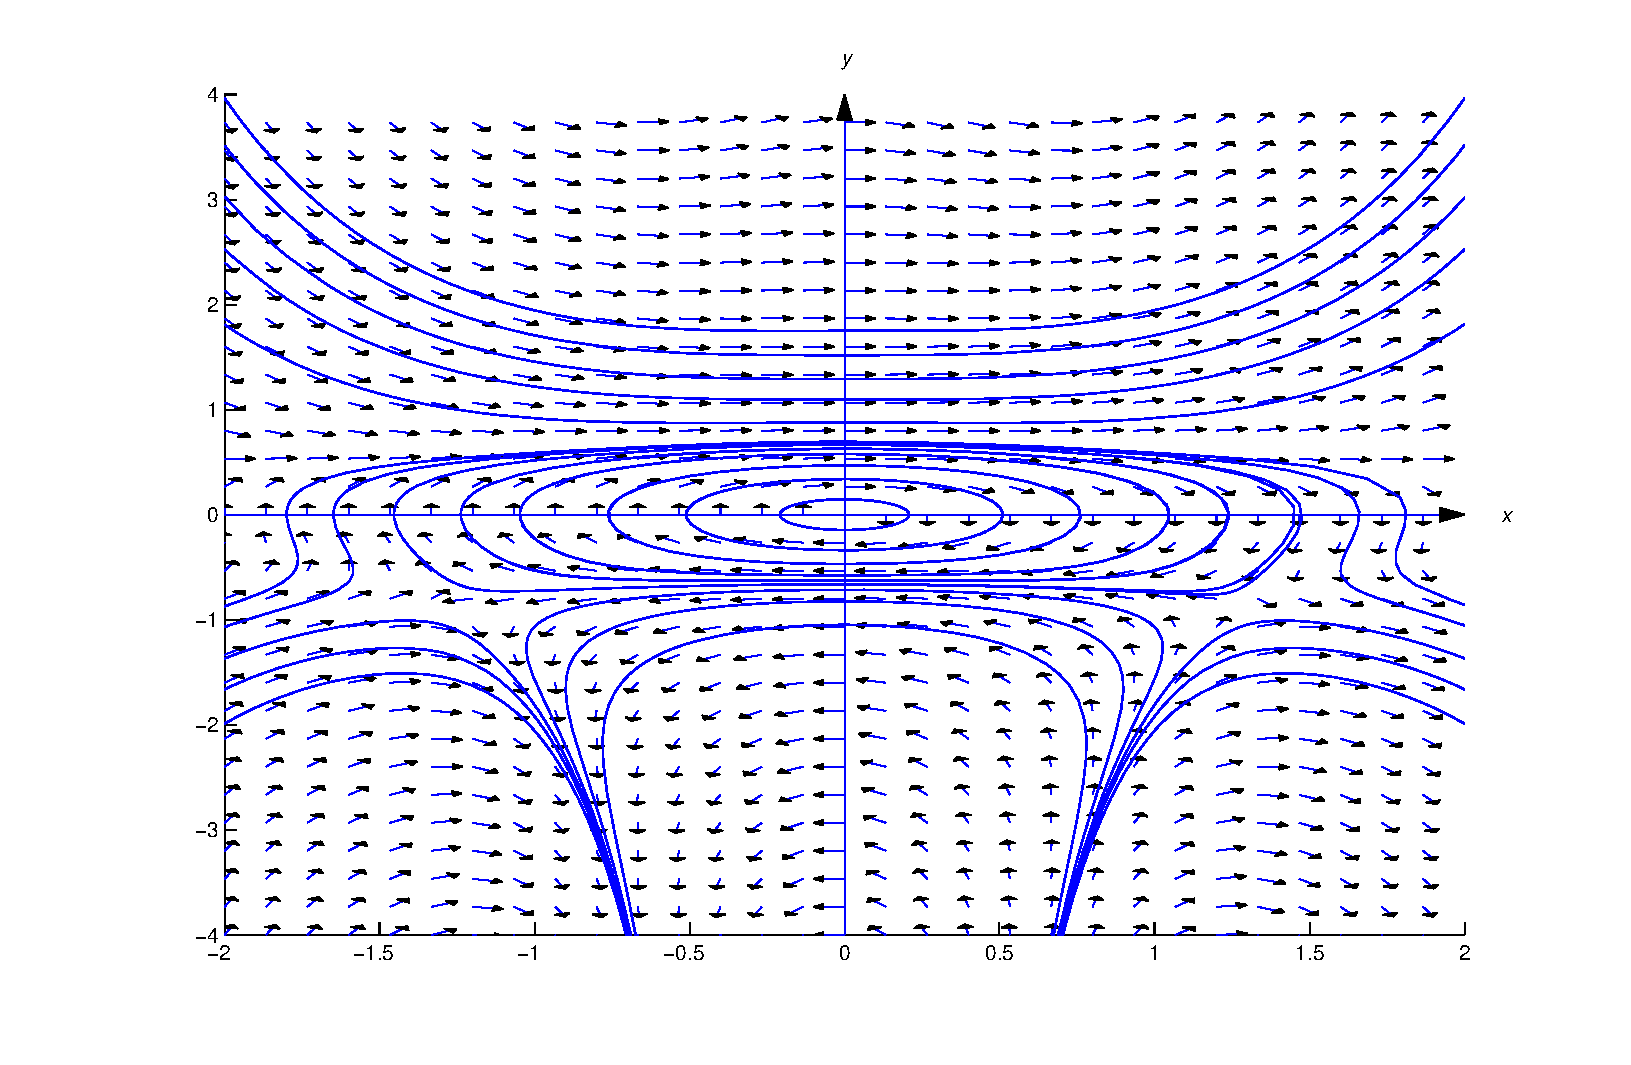
\includegraphics[bb=-78 148 689 643,width=5.67in,height=3.66in,keepaspectratio]{fig020601}
\color{blue}
\caption{A direction field and  integral curves for
$(2xy^3-2x^3y^3-4xy^2+2x)\,dx+(3x^2y^2+4y)\,dy=0$}
  \label{figure:2.6.1}
\end{figure}

\begin{example}\label{example:2.6.2}
\rm  Find an integrating factor for
\begin{equation}\label{eq:2.6.18}
2xy^3\,dx+(3x^2y^2+x^2y^3+1)\,dy=0
\end{equation}
and solve the equation.
\end{example}

\solution In \eqref{eq:2.6.18},
$$
M=2xy^3,\quad N=3x^2y^2+x^2y^3+1,
$$
and
$$
M_y-N_x=6xy^2-(6xy^2+2xy^3)=-2xy^3,
$$
so \eqref{eq:2.6.18} isn't  exact.  Moreover,
$$
{M_y-N_x\over N}=-{2xy^3\over 3x^2y^2+x^2y^2+1}
$$
is not independent of $y$, so Theorem~\ref{thmtype:2.6.1}(a) does not
apply. However,   Theorem~\ref{thmtype:2.6.1}(b) does apply, since
$$
{N_x-M_y\over M}={2xy^3\over 2xy^3}=1
$$
is independent of $x$, so we can take $q(y)=1$.
 Since
$$
\int q(y)\,dy=\int\,dy=y,
$$
  $\mu(y)=e^y$ is
an integrating factor. Multiplying \eqref{eq:2.6.18} by $\mu$ yields the
exact equation
\begin{equation}\label{eq:2.6.19}
2xy^3e^y\,dx+(3x^2y^2+x^2y^3+1)e^y\,dy=0.
\end{equation}
To solve this equation, we must find a
function $F$ such that
\begin{equation}\label{eq:2.6.20}
F_x(x,y)=2xy^3e^y
\end{equation}
 and
\begin{equation}\label{eq:2.6.21}
F_y(x,y)=(3x^2y^2+x^2y^3+1)e^y.
\end{equation}
 Integrating \eqref{eq:2.6.20} with respect to $x$ yields
\begin{equation}\label{eq:2.6.22}
F(x,y)=x^2y^3e^y+\phi(y).
\end{equation}
Differentiating this with respect to $y$ yields
$$
F_y=(3x^2y^2+x^2y^3)e^y+\phi'(y),
$$
and comparing this with \eqref{eq:2.6.21} shows that $\phi'(y)=e^y$.
 Therefore we set $\phi(y)=e^y$ in \eqref{eq:2.6.22} and conclude
that
$$
(x^2y^3+1)e^y=c
$$
is an implicit solution of \eqref{eq:2.6.19}.
It is also an implicit solution
 of \eqref{eq:2.6.18}. Figure~\ref{figure:2.6.2} shows a direction
field and some integral curves for \eqref{eq:2.6.18}.\bbox

           \begin{figure}[H]
  \centering
  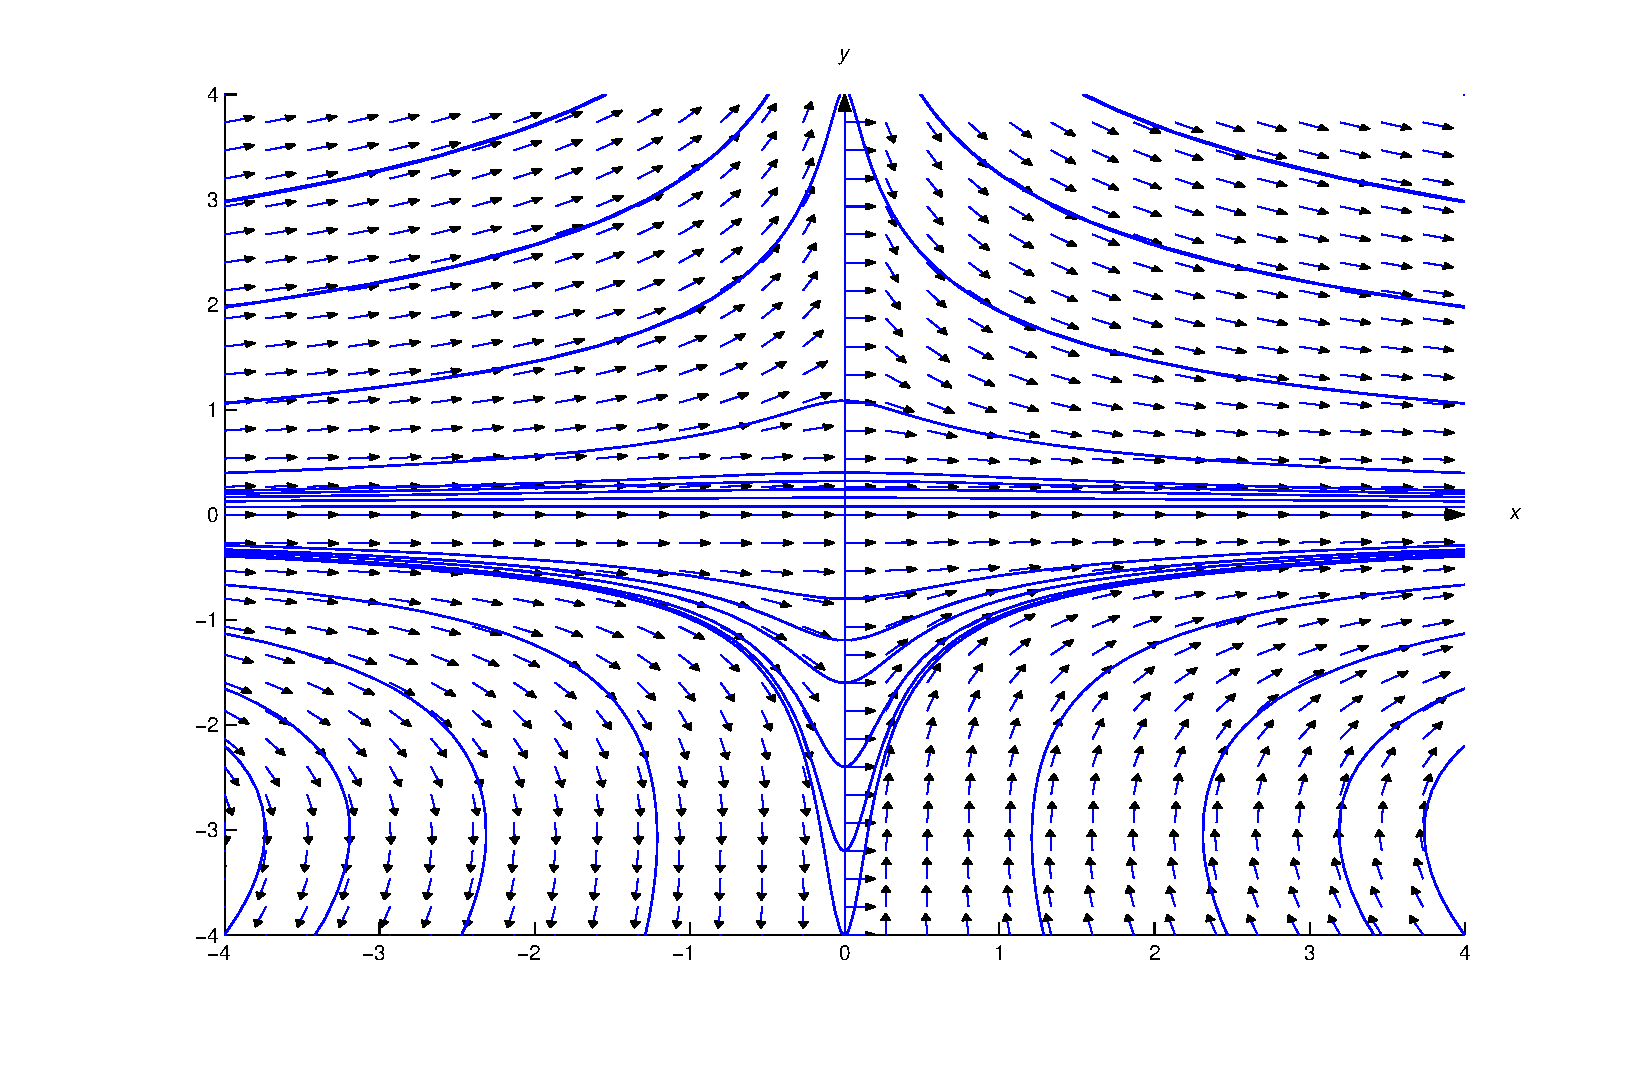
\includegraphics[bb=-78 148 689 643,width=5.67in,height=3.66in,keepaspectratio]{fig020602}
\color{blue}
\caption{
A direction field and integral curves for
$2xy^3e^y\,dx+(3x^2y^2+x^2y^3+1)e^y\,dy=0$}
  \label{figure:2.6.2}
\end{figure}

Theorem~\ref{thmtype:2.6.1} does not apply in the next example,
but the more general argument that led to Theorem~\ref{thmtype:2.6.1}
provides an integrating factor.

\begin{example}\label{example:2.6.3} \rm Find an integrating factor for
\begin{equation}\label{eq:2.6.23}
(3xy+6y^2)\,dx+(2x^2+9xy)\,dy=0
\end{equation} and solve the equation.
 \end{example}

\solution In \eqref{eq:2.6.23}
 $$
 M=3xy+6y^2,\ N=2x^2+9xy,
 $$
and
 $$
M_y-N_x=(3x+12y)-(4x+9y)=-x+3y.
$$
 Therefore
 $$ {M_y-N_x\over
M}={-x+3y\over 3xy+6y^2} \mbox{\quad and \quad} {N_x-M_y\over
N}={x-3y\over 2x^2+9xy},
 $$
so Theorem~\ref{thmtype:2.6.1} does not apply.
Following the more general argument that led to
Theorem~\ref{thmtype:2.6.1}, we look for functions $p=p(x)$ and $q=q(y)$
such that
$$
M_y-N_x=p(x)N-q(y)M;
 $$ that is,
$$
-x+3y=p(x)(2x^2+9xy)-q(y)(3xy+6y^2).
$$
Since the left side contains
only first degree terms in $x$ and $y$, we rewrite this equation as
$$
xp(x)(2x+9y)-yq(y)(3x+6y)=-x+3y.
 $$
 This will be an identity if
\begin{equation}\label{eq:2.6.24}
 xp(x)=A\mbox{\quad and\quad} yq(y)=B,
\end{equation}
 where $A$ and $B$ are constants such that
$$
-x+3y=A(2x+9y)-B(3x+6y),
 $$
 or, equivalently,
$$
-x+3y=(2A-3B)x+(9A-6B)y.
$$
Equating the coefficients of $x$ and $y$
on both sides shows that the last equation holds for all $(x,y)$ if
\begin{eqnarray*} 2A-3B &=&-1 \\ 9A-6B &=&\phantom{-}3,
\end{eqnarray*}
 which has the solution $A=1$, $B=1$. Therefore
\eqref{eq:2.6.24} implies that
 $$ p(x)={1\over x}\mbox{\quad and \quad}
q(y)={1\over y}.
$$
Since
 $$ \int p(x)\,dx=\ln|x|\mbox{\quad
and\quad}\int q(y)\,dy=\ln|y|,
$$
 we can let $P(x)=x$ and $Q(y)=y$;
hence, $\mu(x,y)=xy$ is an integrating factor. Multiplying
\eqref{eq:2.6.23} by $\mu$ yields the exact equation
$$
(3x^2y^2+6xy^3)\,dx+(2x^3y+9x^2y^2)\,dy=0.
 $$
 We leave it to you to
use the method of Section~2.5 to show that this equation has the
implicit solution
\begin{equation}
 \label{eq:2.6.25} x^3y^2+3x^2y^3=c.
\end{equation}
This is also an implicit solution of \eqref{eq:2.6.23}.
Since $x\equiv0$ and $y\equiv0$ satisfy \eqref{eq:2.6.25}, you should
check to see that $x\equiv0$ and $y\equiv0$ are also solutions of
\eqref{eq:2.6.23}. (Why is it necessary to check this?)

Figure~\ref{figure:2.6.3} shows a direction field and integral curves for
\eqref{eq:2.6.23}.

See Exercise~\ref{exer:2.6.28} for a general discussion of equations like
\eqref{eq:2.6.23}.

        \begin{figure}[tbp]
  \centering
  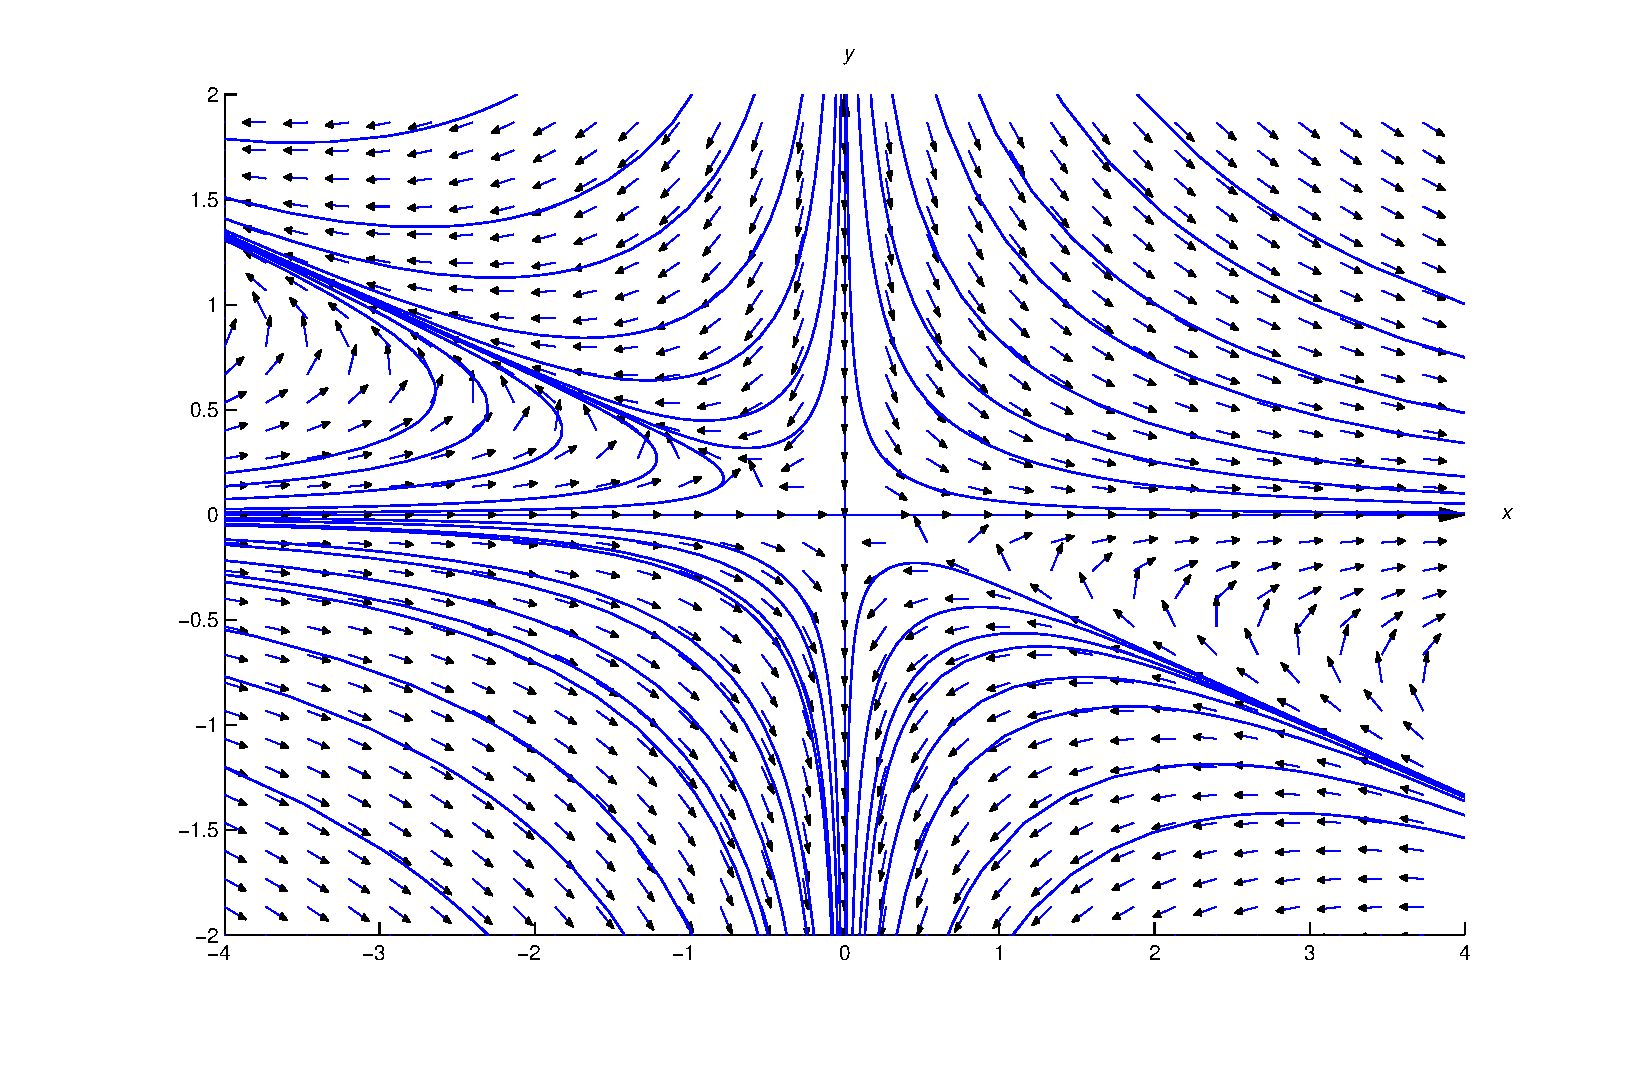
\includegraphics[bb=-78 148 689 643,width=5.67in,height=3.66in,keepaspectratio]{fig020603}
\color{blue}
\caption{
A direction field and integral curves for
$(3xy+6y^2)\,dx+(2x^2+9xy)\,dy=0$}
  \label{figure:2.6.3}
\end{figure}

\begin{example}\label{example:2.6.4}
\rm  The separable  equation
\begin{equation}\label{eq:2.6.26}
-y\,dx+(x+x^6)\,dy=0
\end{equation}
can be converted to the exact equation
\begin{equation} \label{eq:2.6.27}
-{dx\over x+x^6}+{dy\over y}=0
\end{equation}
by multiplying through
by the  integrating factor
$$
\mu(x,y)={1\over y(x+x^6)}.
$$
However, to solve \eqref{eq:2.6.27} by the method of Section~2.5
we would have to evaluate the nasty integral
$$
\int {dx\over x+x^6}.
$$
Instead, we solve \eqref{eq:2.6.26} explicitly for $y$ by finding  an
integrating factor of the form
$\mu(x,y)=x^ay^b$.
\end{example}

\begin{figure}[H]
  \centering
  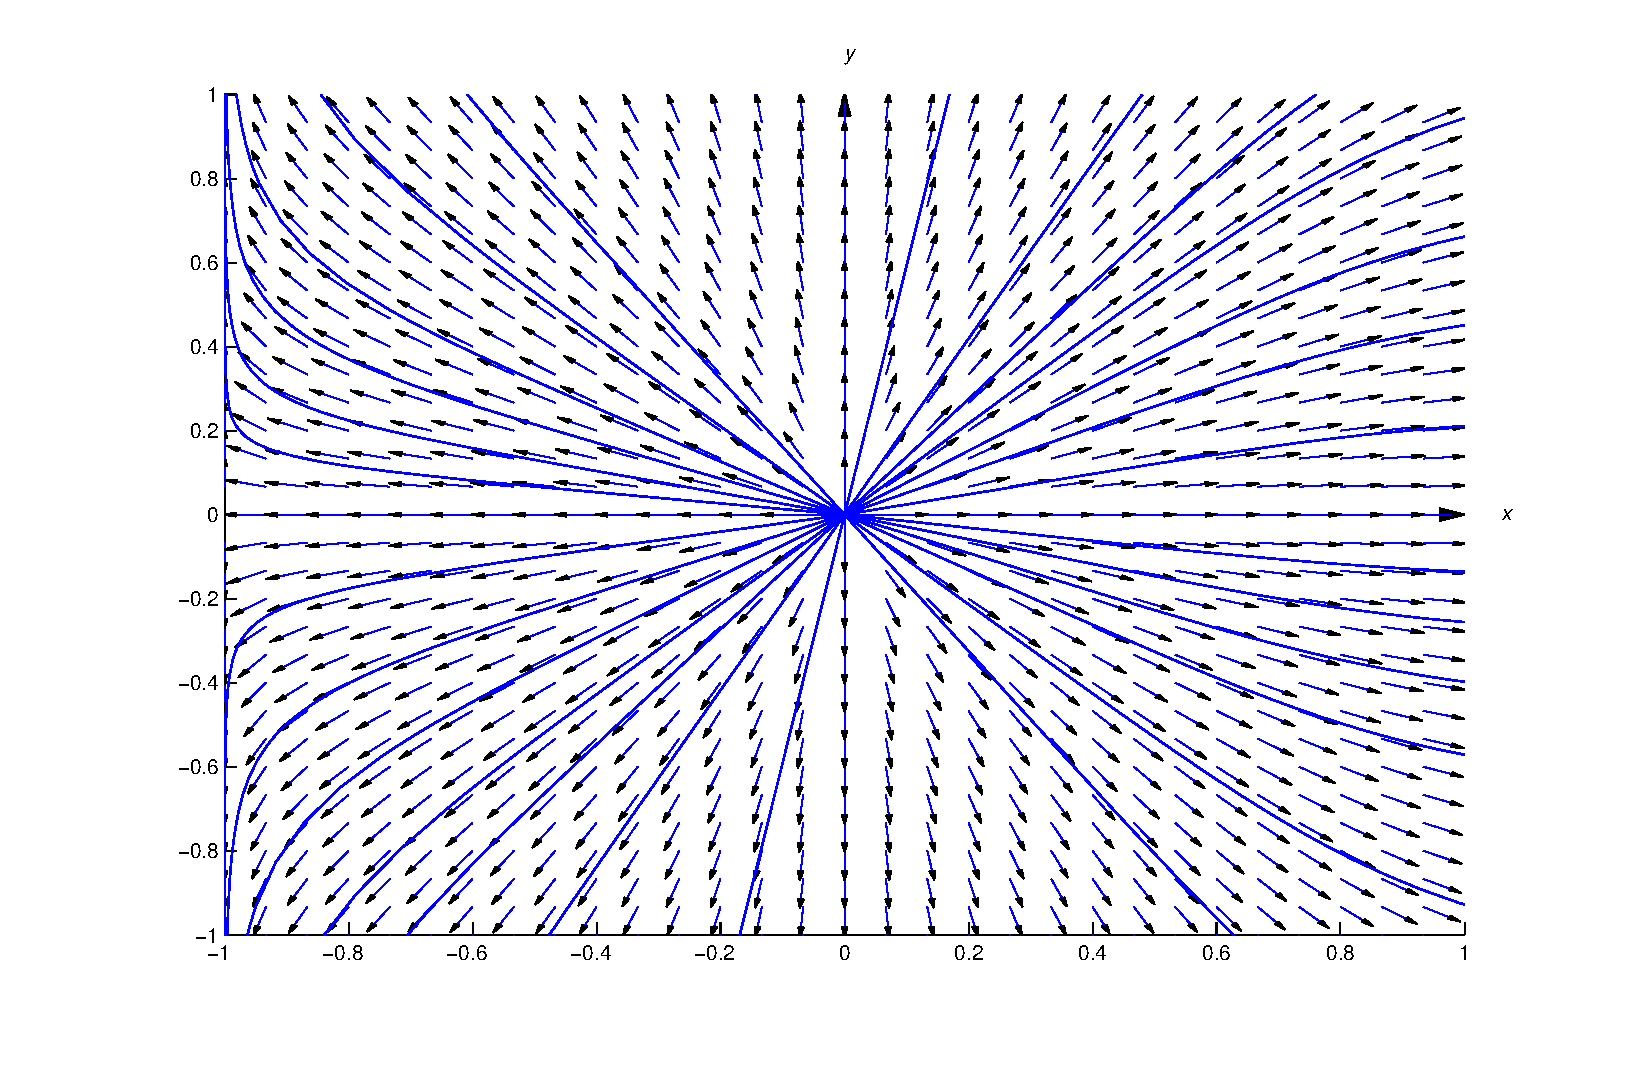
\includegraphics[bb=-78 148 689 643,width=5.67in,height=3.66in,keepaspectratio]{fig020604}
\color{blue}
\caption{A direction field and integral curves for $-y\,dx+(x+x^6)\,dy=0$}
  \label{figure:2.6.4}
\end{figure}

\solution
In \eqref{eq:2.6.26}
$$
M=-y,\ N=x+x^6,
$$
and
$$
M_y-N_x=-1-(1+6x^5)=-2-6x^5.
$$
We  look for functions
$p=p(x)$ and $q=q(y)$ such that
$$
M_y-N_x=p(x)N-q(y)M;
$$
that is,
\begin{equation}\label{eq:2.6.28}
-2-6x^5=p(x)(x+x^6)+q(y)y.
\end{equation}
The right side will contain the term $-6x^5$ if $p(x)=-6/x$.   Then
\eqref{eq:2.6.28} becomes
$$
-2-6x^5=-6-6x^5+q(y)y,
$$
so  $q(y)=4/y$.  Since
$$
\int p(x)\,dx=-\int{6\over x}\,dx=-6\ln|x|=\ln{1\over x^6},
$$
 and
$$
\int q(y)\,dy=\int{4\over y}\,dy=4\ln
|y|=\ln{y^4},
$$
we can take $P(x)=x^{-6}$ and $Q(y)=y^4$,
which yields the integrating factor $\mu(x,y)=x^{-6}y^4$.
Multiplying \eqref{eq:2.6.26} by  $\mu$ yields the exact equation
$$
-{y^5\over x^6}\,dx+\left({y^4\over x^5}+y^4\right)
\,dy=0.
$$
 We leave it to you to use the method of the Section~2.5
to show that this equation has the implicit solution $$
\left({y\over x}\right)^5+y^5=k.
$$
 Solving for $y$ yields
$$
y=k^{1/5}x(1+x^5)^{-1/5},
$$
which we rewrite as
$$
y=cx(1+x^5)^{-1/5}
$$
by renaming the arbitrary constant.
 This is also a solution of \eqref{eq:2.6.26}.

Figure~\ref{figure:2.6.4} shows a direction field and some integral curves
 for \eqref{eq:2.6.26}.

 \exercises
\begin{exerciselist}

\item\label{exer:2.6.1}
\begin{alist}
\item % (a)
Verify that $\mu(x,y)=y$ is an integrating factor for
$$
y\,dx+\left(2x+{1\over y}\right)\,dy=0
\eqno{\rm (A)}
$$
on any open rectangle that does not intersect  the $x$ axis
or, equivalently,  that
$$
y^2\,dx+(2xy+1)\,dy=0
\eqno{\rm (B)}
$$
is exact on any such rectangle.
\item % (b)
Verify that $y\equiv0$  is a solution of  (B),
but not of  (A).
\item % (b)
Show that
$$
y(xy+1)=c
\eqno{\rm (C)}
$$
is an implicit solution of (B), and explain why
every differentiable function $y=y(x)$ other than $y\equiv0$
that satisfies  (C)
 is also a solution of~(A).
\end{alist}

\item\label{exer:2.6.2}
\begin{alist}
\item % (a)
Verify that $\mu(x,y)=1/(x-y)^2$ is an integrating factor for
$$
-y^2\,dx+x^2\,dy=0
\eqno{\rm (A)}
$$
on any open rectangle  that does not intersect the line $y=x$
or, equivalently, that
$$
-{y^2\over(x-y)^2}\,dx+{x^2\over(x-y)^2}\,dy=0
\eqno{\rm (B)}
$$
is exact on any such rectangle.
\item % (b)
Use Theorem~\ref{thmtype:2.2.1} to show that
$$
{xy\over(x-y)}=c
\eqno{\rm (C)}
$$
is an implicit solution of (B), and explain why
it's also an implicit solution of (A)
\item % (b)
Verify that $y=x$  is a solution of  (A),
even though it can't be obtained from  (C).
\end{alist}

\exercisetext{In Exercises~\ref{exer:2.6.3}--\ref{exer:2.6.16} find an
integrating factor;
that is a function of only one variable, and solve the given equation.}

\begin{tabular}[t]{@{}p{168pt}@{}p{168pt}}
\item\label{exer:2.6.3} $y\,dx-x\,dy=0$ &
\item\label{exer:2.6.4} \vspace*{7.5pt} $3x^2y\,dx+2x^3\,dy=0$
\end{tabular}

\begin{tabular}[t]{@{}p{168pt}@{}p{168pt}}
\item\label{exer:2.6.5} $2y^3\,dx+3y^2\,dy=0$&
\item\label{exer:2.6.6} $(5xy+2y+5)\,dx+2x\,dy=0$
\end{tabular}

\item\label{exer:2.6.7} $(xy+x+2y+1)\,dx+(x+1)\,dy=0$

\item\label{exer:2.6.8} $(27xy^2+8y^3)\,dx+(18x^2y+12xy^2)\,dy=0$

\item\label{exer:2.6.9} $(6xy^2+2y)\,dx+(12x^2y+6x+3)\,dy=0$

\item\label{exer:2.6.10} $y^2\,dx+\dst{\left(xy^2+3xy+{1\over
y}\right)\,dy=0}$

\item\label{exer:2.6.11} $(12x^3y+24x^2y^2)\,dx+(9x^4+32x^3y+4y)\,dy=0$

\item\label{exer:2.6.12} $(x^2y+4xy+2y)\,dx+(x^2+x)\,dy=0$

\item\label{exer:2.6.13} $-y\,dx+(x^4-x)\,dy=0$

\item\label{exer:2.6.14} $\cos x\cos y\,dx
+(\sin x\cos y-\sin x\sin y+y)\,dy=0$

\item\label{exer:2.6.15} $(2xy+y^2)\,dx+(2xy+x^2-2x^2y^2-2xy^3)\,dy=0$

\item\label{exer:2.6.16} $y\sin y\,dx+x(\sin y-y\cos y)\,dy=0$

\exercisetext{In Exercises~\ref{exer:2.6.17}--\ref{exer:2.6.23} find an
integrating
factor of the form $\mu(x,y)=P(x)Q(y)$ and solve the given equation.}

\item\label{exer:2.6.17}
$y(1+5\ln|x|)\,dx+4x\ln|x|\,dy=0$

 \item\label{exer:2.6.18}
 $(\alpha y+ \gamma xy)\,dx+(\beta x+ \delta xy)\,dy=0$

\item\label{exer:2.6.19}
$(3x^2y^3-y^2+y)\,dx+(-xy+2x)\,dy=0$

\item\label{exer:2.6.20} $2y\,dx+ 3(x^2+x^2y^3)\,dy=0$

\item\label{exer:2.6.21}
$(a\cos xy-y\sin xy)\,dx+(b\cos xy-x\sin xy)\,
dy=0$

\item\label{exer:2.6.22}
$x^4y^4\,dx+x^5y^3\,dy=0$

\item\label{exer:2.6.23}
$y(x\cos x+2\sin x)\,dx+x(y+1)\sin x\,dy=0$

\exercisetext{In Exercises~\ref{exer:2.6.24}--\ref{exer:2.6.27} find an
integrating factor
and solve the  equation. Plot a direction field and some
integral curves for the equation in the indicated rectangular region.}

\item\label{exer:2.6.24} \CGex
 $(x^4y^3+y)\,dx+(x^5y^2-x)\,dy=0;   \quad \{-1\le x\le1,-1\le y\le1\}$

\item\label{exer:2.6.25} \CGex
$(3xy+2y^2+y)\,dx+(x^2+2xy+x+2y)\,dy=0;   \quad \{-2\le x\le2,-2\le
y\le2\}$

\item\label{exer:2.6.26} \CGex
$(12 xy+6y^3)\,dx+(9x^2+10xy^2)\,dy=0;   \quad \{-2\le x\le2,-2\le y\le2\}$

\item\label{exer:2.6.27} \CGex
$(3x^2y^2+2y)\,dx+ 2x\,dy=0;   \quad \{-4\le x\le4,-4\le y\le4\}$

\item\label{exer:2.6.28}
Suppose $a$, $b$, $c$, and $d$ are constants such that
$ad-bc\ne0$, and let $m$ and $n$ be arbitrary real numbers.
Show that
$$
(ax^my+by^{n+1})\,dx+(cx^{m+1}+dxy^n)\,dy=0
$$
has an integrating factor $\mu(x,y)=x^\alpha y^\beta$.

\item\label{exer:2.6.29}
Suppose $M$, $N$, $M_x$, and $N_y$  are continuous for all
$(x,y)$, and $\mu=\mu(x,y)$  is an integrating factor for
$$
M(x,y)\,dx+N(x,y)\,dy=0.
\eqno{\rm (A)}
$$
Assume that $\mu_x$ and $\mu_y$ are continuous for all $(x,y)$, and
suppose   $y=y(x)$ is a differentiable function such that
$\mu(x,y(x))=0$ and $\mu_x(x,y(x))\ne0$ for all $x$ in some interval
$I$. Show that $y$ is a solution of (A) on $I$.

\item\label{exer:2.6.30}
According to Theorem~\ref{thmtype:2.1.2}, the general solution of the
linear nonhomogeneous equation
$$
y'+p(x)y=f(x)
\eqno{\rm(A)}
$$
is
$$
y=y_1(x)\left(c+\int f(x)/y_1(x)\,dx\right),
\eqno{\rm(B)}
$$
where $y_1$ is any nontrivial solution of the
complementary equation $y'+p(x)y=0$. In this exercise we obtain this
conclusion in a different way.
You may find it instructive to apply the method suggested here
to solve some of the exercises in Section~2.1.
\begin{alist}
\item % (a)
Rewrite (A) as
$$
[p(x)y-f(x)]\,dx+\,dy=0,
\eqno{\rm(C)}
$$
and show that $\mu=\pm e^{\int p(x)\,dx}$ is an integrating factor
for (C).
\item % (b)
Multiply (A) through by $\mu=\pm e^{\int p(x)\,dx}$  and verify that
the resulting equation can be rewritten as
$$
(\mu(x)y)'=\mu(x)f(x).
$$
Then integrate both sides of this equation and solve for $y$
to show that the general solution of (A) is
$$
y={1\over\mu(x)}\left(c+\int f(x)\mu(x)\,dx\right).
$$
Why is this form of the general solution
 equivalent to (B)?
\end{alist}

\end{exerciselist}

